\section*{GBM}

Gradient Boosting Method is an agorithm that is part of ensemble methods. See associated \hyperref[sec:ensemble-methods]{section} for the details.

There are many different implementation of this method; the below one (src: Wikipedia) is one of the most generic and understandable.

\begin{center}
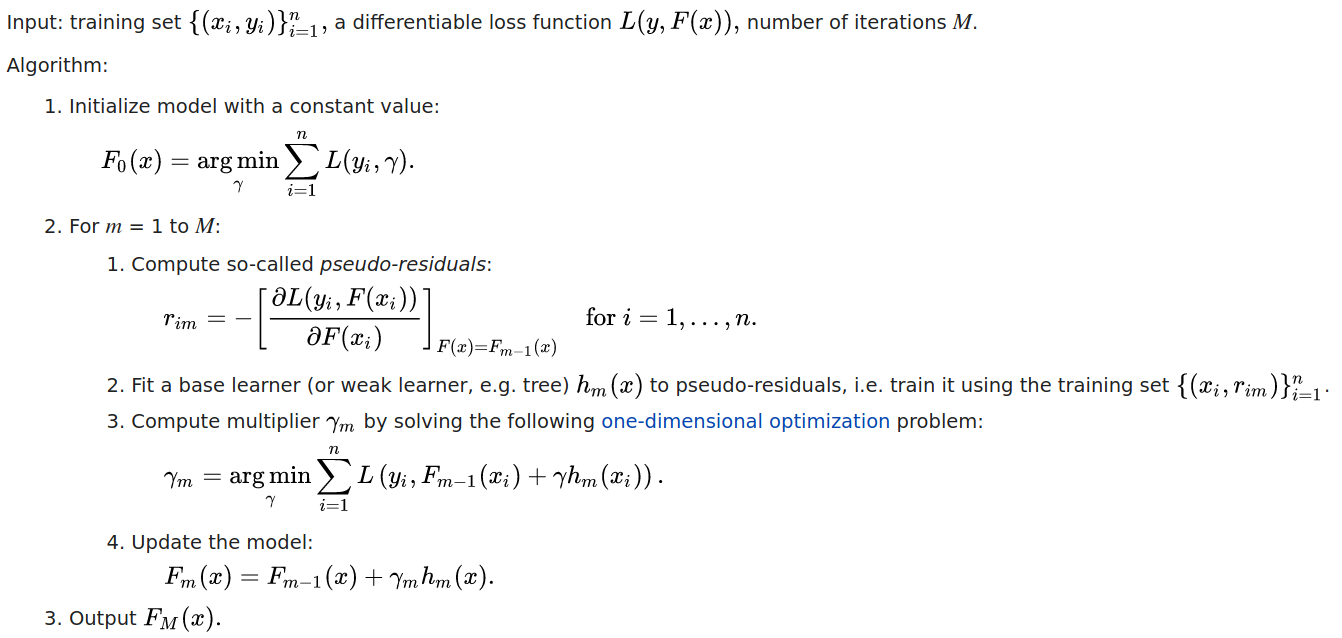
\includegraphics[scale=0.3]{GBM_algo.png}
\end{center}

\underline{Step 1: initialize model with constant value}

$$F_0 = \underset{\hat y}{argmin} \Sigma_{i=1}^n \mathcal{L}(y,\hat y)$$

We note that $\hat y$ is constant and doesn't depend on $i$. Consequently, optimizing this equation using MSE as loss function will lead to $\hat y = \bar y$:

$MSE = \frac{1}{n}\Sigma_{i=1}^n (y_i - \hat y)^2$

$\frac{\partial \mathcal{L}}{\partial \hat y} = 0$

=> $\frac{2}{n}(y_1 - \hat y) + ... + (y_n - \hat y) = 0$

=> $\hat y = \Sigma_{i=1}^n \frac{y_i}{n}$

\underline{Step 2: loop on the number of estimators} \\

\textit{Pseudo-residuals} \\






Implementation from scratch - comments

Parameters to optimize

\vspace{5mm}